
% Default to the notebook output style

    


% Inherit from the specified cell style.




    
\documentclass[11pt]{article}

    
    
    \usepackage[T1]{fontenc}
    % Nicer default font (+ math font) than Computer Modern for most use cases
    \usepackage{mathpazo}

    % Basic figure setup, for now with no caption control since it's done
    % automatically by Pandoc (which extracts ![](path) syntax from Markdown).
    \usepackage{graphicx}
    % We will generate all images so they have a width \maxwidth. This means
    % that they will get their normal width if they fit onto the page, but
    % are scaled down if they would overflow the margins.
    \makeatletter
    \def\maxwidth{\ifdim\Gin@nat@width>\linewidth\linewidth
    \else\Gin@nat@width\fi}
    \makeatother
    \let\Oldincludegraphics\includegraphics
    % Set max figure width to be 80% of text width, for now hardcoded.
    \renewcommand{\includegraphics}[1]{\Oldincludegraphics[width=.8\maxwidth]{#1}}
    % Ensure that by default, figures have no caption (until we provide a
    % proper Figure object with a Caption API and a way to capture that
    % in the conversion process - todo).
    \usepackage{caption}
    \DeclareCaptionLabelFormat{nolabel}{}
    \captionsetup{labelformat=nolabel}

    \usepackage{adjustbox} % Used to constrain images to a maximum size 
    \usepackage{xcolor} % Allow colors to be defined
    \usepackage{enumerate} % Needed for markdown enumerations to work
    \usepackage{geometry} % Used to adjust the document margins
    \usepackage{amsmath} % Equations
    \usepackage{amssymb} % Equations
    \usepackage{textcomp} % defines textquotesingle
    % Hack from http://tex.stackexchange.com/a/47451/13684:
    \AtBeginDocument{%
        \def\PYZsq{\textquotesingle}% Upright quotes in Pygmentized code
    }
    \usepackage{upquote} % Upright quotes for verbatim code
    \usepackage{eurosym} % defines \euro
    \usepackage[mathletters]{ucs} % Extended unicode (utf-8) support
    \usepackage[utf8x]{inputenc} % Allow utf-8 characters in the tex document
    \usepackage{fancyvrb} % verbatim replacement that allows latex
    \usepackage{grffile} % extends the file name processing of package graphics 
                         % to support a larger range 
    % The hyperref package gives us a pdf with properly built
    % internal navigation ('pdf bookmarks' for the table of contents,
    % internal cross-reference links, web links for URLs, etc.)
    \usepackage{hyperref}
    \usepackage{longtable} % longtable support required by pandoc >1.10
    \usepackage{booktabs}  % table support for pandoc > 1.12.2
    \usepackage[inline]{enumitem} % IRkernel/repr support (it uses the enumerate* environment)
    \usepackage[normalem]{ulem} % ulem is needed to support strikethroughs (\sout)
                                % normalem makes italics be italics, not underlines
    

    
    
    % Colors for the hyperref package
    \definecolor{urlcolor}{rgb}{0,.145,.698}
    \definecolor{linkcolor}{rgb}{.71,0.21,0.01}
    \definecolor{citecolor}{rgb}{.12,.54,.11}

    % ANSI colors
    \definecolor{ansi-black}{HTML}{3E424D}
    \definecolor{ansi-black-intense}{HTML}{282C36}
    \definecolor{ansi-red}{HTML}{E75C58}
    \definecolor{ansi-red-intense}{HTML}{B22B31}
    \definecolor{ansi-green}{HTML}{00A250}
    \definecolor{ansi-green-intense}{HTML}{007427}
    \definecolor{ansi-yellow}{HTML}{DDB62B}
    \definecolor{ansi-yellow-intense}{HTML}{B27D12}
    \definecolor{ansi-blue}{HTML}{208FFB}
    \definecolor{ansi-blue-intense}{HTML}{0065CA}
    \definecolor{ansi-magenta}{HTML}{D160C4}
    \definecolor{ansi-magenta-intense}{HTML}{A03196}
    \definecolor{ansi-cyan}{HTML}{60C6C8}
    \definecolor{ansi-cyan-intense}{HTML}{258F8F}
    \definecolor{ansi-white}{HTML}{C5C1B4}
    \definecolor{ansi-white-intense}{HTML}{A1A6B2}

    % commands and environments needed by pandoc snippets
    % extracted from the output of `pandoc -s`
    \providecommand{\tightlist}{%
      \setlength{\itemsep}{0pt}\setlength{\parskip}{0pt}}
    \DefineVerbatimEnvironment{Highlighting}{Verbatim}{commandchars=\\\{\}}
    % Add ',fontsize=\small' for more characters per line
    \newenvironment{Shaded}{}{}
    \newcommand{\KeywordTok}[1]{\textcolor[rgb]{0.00,0.44,0.13}{\textbf{{#1}}}}
    \newcommand{\DataTypeTok}[1]{\textcolor[rgb]{0.56,0.13,0.00}{{#1}}}
    \newcommand{\DecValTok}[1]{\textcolor[rgb]{0.25,0.63,0.44}{{#1}}}
    \newcommand{\BaseNTok}[1]{\textcolor[rgb]{0.25,0.63,0.44}{{#1}}}
    \newcommand{\FloatTok}[1]{\textcolor[rgb]{0.25,0.63,0.44}{{#1}}}
    \newcommand{\CharTok}[1]{\textcolor[rgb]{0.25,0.44,0.63}{{#1}}}
    \newcommand{\StringTok}[1]{\textcolor[rgb]{0.25,0.44,0.63}{{#1}}}
    \newcommand{\CommentTok}[1]{\textcolor[rgb]{0.38,0.63,0.69}{\textit{{#1}}}}
    \newcommand{\OtherTok}[1]{\textcolor[rgb]{0.00,0.44,0.13}{{#1}}}
    \newcommand{\AlertTok}[1]{\textcolor[rgb]{1.00,0.00,0.00}{\textbf{{#1}}}}
    \newcommand{\FunctionTok}[1]{\textcolor[rgb]{0.02,0.16,0.49}{{#1}}}
    \newcommand{\RegionMarkerTok}[1]{{#1}}
    \newcommand{\ErrorTok}[1]{\textcolor[rgb]{1.00,0.00,0.00}{\textbf{{#1}}}}
    \newcommand{\NormalTok}[1]{{#1}}
    
    % Additional commands for more recent versions of Pandoc
    \newcommand{\ConstantTok}[1]{\textcolor[rgb]{0.53,0.00,0.00}{{#1}}}
    \newcommand{\SpecialCharTok}[1]{\textcolor[rgb]{0.25,0.44,0.63}{{#1}}}
    \newcommand{\VerbatimStringTok}[1]{\textcolor[rgb]{0.25,0.44,0.63}{{#1}}}
    \newcommand{\SpecialStringTok}[1]{\textcolor[rgb]{0.73,0.40,0.53}{{#1}}}
    \newcommand{\ImportTok}[1]{{#1}}
    \newcommand{\DocumentationTok}[1]{\textcolor[rgb]{0.73,0.13,0.13}{\textit{{#1}}}}
    \newcommand{\AnnotationTok}[1]{\textcolor[rgb]{0.38,0.63,0.69}{\textbf{\textit{{#1}}}}}
    \newcommand{\CommentVarTok}[1]{\textcolor[rgb]{0.38,0.63,0.69}{\textbf{\textit{{#1}}}}}
    \newcommand{\VariableTok}[1]{\textcolor[rgb]{0.10,0.09,0.49}{{#1}}}
    \newcommand{\ControlFlowTok}[1]{\textcolor[rgb]{0.00,0.44,0.13}{\textbf{{#1}}}}
    \newcommand{\OperatorTok}[1]{\textcolor[rgb]{0.40,0.40,0.40}{{#1}}}
    \newcommand{\BuiltInTok}[1]{{#1}}
    \newcommand{\ExtensionTok}[1]{{#1}}
    \newcommand{\PreprocessorTok}[1]{\textcolor[rgb]{0.74,0.48,0.00}{{#1}}}
    \newcommand{\AttributeTok}[1]{\textcolor[rgb]{0.49,0.56,0.16}{{#1}}}
    \newcommand{\InformationTok}[1]{\textcolor[rgb]{0.38,0.63,0.69}{\textbf{\textit{{#1}}}}}
    \newcommand{\WarningTok}[1]{\textcolor[rgb]{0.38,0.63,0.69}{\textbf{\textit{{#1}}}}}
    
    
    % Define a nice break command that doesn't care if a line doesn't already
    % exist.
    \def\br{\hspace*{\fill} \\* }
    % Math Jax compatability definitions
    \def\gt{>}
    \def\lt{<}
    % Document parameters
    \title{Raport}
    
    
    

    % Pygments definitions
    
\makeatletter
\def\PY@reset{\let\PY@it=\relax \let\PY@bf=\relax%
    \let\PY@ul=\relax \let\PY@tc=\relax%
    \let\PY@bc=\relax \let\PY@ff=\relax}
\def\PY@tok#1{\csname PY@tok@#1\endcsname}
\def\PY@toks#1+{\ifx\relax#1\empty\else%
    \PY@tok{#1}\expandafter\PY@toks\fi}
\def\PY@do#1{\PY@bc{\PY@tc{\PY@ul{%
    \PY@it{\PY@bf{\PY@ff{#1}}}}}}}
\def\PY#1#2{\PY@reset\PY@toks#1+\relax+\PY@do{#2}}

\expandafter\def\csname PY@tok@w\endcsname{\def\PY@tc##1{\textcolor[rgb]{0.73,0.73,0.73}{##1}}}
\expandafter\def\csname PY@tok@c\endcsname{\let\PY@it=\textit\def\PY@tc##1{\textcolor[rgb]{0.25,0.50,0.50}{##1}}}
\expandafter\def\csname PY@tok@cp\endcsname{\def\PY@tc##1{\textcolor[rgb]{0.74,0.48,0.00}{##1}}}
\expandafter\def\csname PY@tok@k\endcsname{\let\PY@bf=\textbf\def\PY@tc##1{\textcolor[rgb]{0.00,0.50,0.00}{##1}}}
\expandafter\def\csname PY@tok@kp\endcsname{\def\PY@tc##1{\textcolor[rgb]{0.00,0.50,0.00}{##1}}}
\expandafter\def\csname PY@tok@kt\endcsname{\def\PY@tc##1{\textcolor[rgb]{0.69,0.00,0.25}{##1}}}
\expandafter\def\csname PY@tok@o\endcsname{\def\PY@tc##1{\textcolor[rgb]{0.40,0.40,0.40}{##1}}}
\expandafter\def\csname PY@tok@ow\endcsname{\let\PY@bf=\textbf\def\PY@tc##1{\textcolor[rgb]{0.67,0.13,1.00}{##1}}}
\expandafter\def\csname PY@tok@nb\endcsname{\def\PY@tc##1{\textcolor[rgb]{0.00,0.50,0.00}{##1}}}
\expandafter\def\csname PY@tok@nf\endcsname{\def\PY@tc##1{\textcolor[rgb]{0.00,0.00,1.00}{##1}}}
\expandafter\def\csname PY@tok@nc\endcsname{\let\PY@bf=\textbf\def\PY@tc##1{\textcolor[rgb]{0.00,0.00,1.00}{##1}}}
\expandafter\def\csname PY@tok@nn\endcsname{\let\PY@bf=\textbf\def\PY@tc##1{\textcolor[rgb]{0.00,0.00,1.00}{##1}}}
\expandafter\def\csname PY@tok@ne\endcsname{\let\PY@bf=\textbf\def\PY@tc##1{\textcolor[rgb]{0.82,0.25,0.23}{##1}}}
\expandafter\def\csname PY@tok@nv\endcsname{\def\PY@tc##1{\textcolor[rgb]{0.10,0.09,0.49}{##1}}}
\expandafter\def\csname PY@tok@no\endcsname{\def\PY@tc##1{\textcolor[rgb]{0.53,0.00,0.00}{##1}}}
\expandafter\def\csname PY@tok@nl\endcsname{\def\PY@tc##1{\textcolor[rgb]{0.63,0.63,0.00}{##1}}}
\expandafter\def\csname PY@tok@ni\endcsname{\let\PY@bf=\textbf\def\PY@tc##1{\textcolor[rgb]{0.60,0.60,0.60}{##1}}}
\expandafter\def\csname PY@tok@na\endcsname{\def\PY@tc##1{\textcolor[rgb]{0.49,0.56,0.16}{##1}}}
\expandafter\def\csname PY@tok@nt\endcsname{\let\PY@bf=\textbf\def\PY@tc##1{\textcolor[rgb]{0.00,0.50,0.00}{##1}}}
\expandafter\def\csname PY@tok@nd\endcsname{\def\PY@tc##1{\textcolor[rgb]{0.67,0.13,1.00}{##1}}}
\expandafter\def\csname PY@tok@s\endcsname{\def\PY@tc##1{\textcolor[rgb]{0.73,0.13,0.13}{##1}}}
\expandafter\def\csname PY@tok@sd\endcsname{\let\PY@it=\textit\def\PY@tc##1{\textcolor[rgb]{0.73,0.13,0.13}{##1}}}
\expandafter\def\csname PY@tok@si\endcsname{\let\PY@bf=\textbf\def\PY@tc##1{\textcolor[rgb]{0.73,0.40,0.53}{##1}}}
\expandafter\def\csname PY@tok@se\endcsname{\let\PY@bf=\textbf\def\PY@tc##1{\textcolor[rgb]{0.73,0.40,0.13}{##1}}}
\expandafter\def\csname PY@tok@sr\endcsname{\def\PY@tc##1{\textcolor[rgb]{0.73,0.40,0.53}{##1}}}
\expandafter\def\csname PY@tok@ss\endcsname{\def\PY@tc##1{\textcolor[rgb]{0.10,0.09,0.49}{##1}}}
\expandafter\def\csname PY@tok@sx\endcsname{\def\PY@tc##1{\textcolor[rgb]{0.00,0.50,0.00}{##1}}}
\expandafter\def\csname PY@tok@m\endcsname{\def\PY@tc##1{\textcolor[rgb]{0.40,0.40,0.40}{##1}}}
\expandafter\def\csname PY@tok@gh\endcsname{\let\PY@bf=\textbf\def\PY@tc##1{\textcolor[rgb]{0.00,0.00,0.50}{##1}}}
\expandafter\def\csname PY@tok@gu\endcsname{\let\PY@bf=\textbf\def\PY@tc##1{\textcolor[rgb]{0.50,0.00,0.50}{##1}}}
\expandafter\def\csname PY@tok@gd\endcsname{\def\PY@tc##1{\textcolor[rgb]{0.63,0.00,0.00}{##1}}}
\expandafter\def\csname PY@tok@gi\endcsname{\def\PY@tc##1{\textcolor[rgb]{0.00,0.63,0.00}{##1}}}
\expandafter\def\csname PY@tok@gr\endcsname{\def\PY@tc##1{\textcolor[rgb]{1.00,0.00,0.00}{##1}}}
\expandafter\def\csname PY@tok@ge\endcsname{\let\PY@it=\textit}
\expandafter\def\csname PY@tok@gs\endcsname{\let\PY@bf=\textbf}
\expandafter\def\csname PY@tok@gp\endcsname{\let\PY@bf=\textbf\def\PY@tc##1{\textcolor[rgb]{0.00,0.00,0.50}{##1}}}
\expandafter\def\csname PY@tok@go\endcsname{\def\PY@tc##1{\textcolor[rgb]{0.53,0.53,0.53}{##1}}}
\expandafter\def\csname PY@tok@gt\endcsname{\def\PY@tc##1{\textcolor[rgb]{0.00,0.27,0.87}{##1}}}
\expandafter\def\csname PY@tok@err\endcsname{\def\PY@bc##1{\setlength{\fboxsep}{0pt}\fcolorbox[rgb]{1.00,0.00,0.00}{1,1,1}{\strut ##1}}}
\expandafter\def\csname PY@tok@kc\endcsname{\let\PY@bf=\textbf\def\PY@tc##1{\textcolor[rgb]{0.00,0.50,0.00}{##1}}}
\expandafter\def\csname PY@tok@kd\endcsname{\let\PY@bf=\textbf\def\PY@tc##1{\textcolor[rgb]{0.00,0.50,0.00}{##1}}}
\expandafter\def\csname PY@tok@kn\endcsname{\let\PY@bf=\textbf\def\PY@tc##1{\textcolor[rgb]{0.00,0.50,0.00}{##1}}}
\expandafter\def\csname PY@tok@kr\endcsname{\let\PY@bf=\textbf\def\PY@tc##1{\textcolor[rgb]{0.00,0.50,0.00}{##1}}}
\expandafter\def\csname PY@tok@bp\endcsname{\def\PY@tc##1{\textcolor[rgb]{0.00,0.50,0.00}{##1}}}
\expandafter\def\csname PY@tok@fm\endcsname{\def\PY@tc##1{\textcolor[rgb]{0.00,0.00,1.00}{##1}}}
\expandafter\def\csname PY@tok@vc\endcsname{\def\PY@tc##1{\textcolor[rgb]{0.10,0.09,0.49}{##1}}}
\expandafter\def\csname PY@tok@vg\endcsname{\def\PY@tc##1{\textcolor[rgb]{0.10,0.09,0.49}{##1}}}
\expandafter\def\csname PY@tok@vi\endcsname{\def\PY@tc##1{\textcolor[rgb]{0.10,0.09,0.49}{##1}}}
\expandafter\def\csname PY@tok@vm\endcsname{\def\PY@tc##1{\textcolor[rgb]{0.10,0.09,0.49}{##1}}}
\expandafter\def\csname PY@tok@sa\endcsname{\def\PY@tc##1{\textcolor[rgb]{0.73,0.13,0.13}{##1}}}
\expandafter\def\csname PY@tok@sb\endcsname{\def\PY@tc##1{\textcolor[rgb]{0.73,0.13,0.13}{##1}}}
\expandafter\def\csname PY@tok@sc\endcsname{\def\PY@tc##1{\textcolor[rgb]{0.73,0.13,0.13}{##1}}}
\expandafter\def\csname PY@tok@dl\endcsname{\def\PY@tc##1{\textcolor[rgb]{0.73,0.13,0.13}{##1}}}
\expandafter\def\csname PY@tok@s2\endcsname{\def\PY@tc##1{\textcolor[rgb]{0.73,0.13,0.13}{##1}}}
\expandafter\def\csname PY@tok@sh\endcsname{\def\PY@tc##1{\textcolor[rgb]{0.73,0.13,0.13}{##1}}}
\expandafter\def\csname PY@tok@s1\endcsname{\def\PY@tc##1{\textcolor[rgb]{0.73,0.13,0.13}{##1}}}
\expandafter\def\csname PY@tok@mb\endcsname{\def\PY@tc##1{\textcolor[rgb]{0.40,0.40,0.40}{##1}}}
\expandafter\def\csname PY@tok@mf\endcsname{\def\PY@tc##1{\textcolor[rgb]{0.40,0.40,0.40}{##1}}}
\expandafter\def\csname PY@tok@mh\endcsname{\def\PY@tc##1{\textcolor[rgb]{0.40,0.40,0.40}{##1}}}
\expandafter\def\csname PY@tok@mi\endcsname{\def\PY@tc##1{\textcolor[rgb]{0.40,0.40,0.40}{##1}}}
\expandafter\def\csname PY@tok@il\endcsname{\def\PY@tc##1{\textcolor[rgb]{0.40,0.40,0.40}{##1}}}
\expandafter\def\csname PY@tok@mo\endcsname{\def\PY@tc##1{\textcolor[rgb]{0.40,0.40,0.40}{##1}}}
\expandafter\def\csname PY@tok@ch\endcsname{\let\PY@it=\textit\def\PY@tc##1{\textcolor[rgb]{0.25,0.50,0.50}{##1}}}
\expandafter\def\csname PY@tok@cm\endcsname{\let\PY@it=\textit\def\PY@tc##1{\textcolor[rgb]{0.25,0.50,0.50}{##1}}}
\expandafter\def\csname PY@tok@cpf\endcsname{\let\PY@it=\textit\def\PY@tc##1{\textcolor[rgb]{0.25,0.50,0.50}{##1}}}
\expandafter\def\csname PY@tok@c1\endcsname{\let\PY@it=\textit\def\PY@tc##1{\textcolor[rgb]{0.25,0.50,0.50}{##1}}}
\expandafter\def\csname PY@tok@cs\endcsname{\let\PY@it=\textit\def\PY@tc##1{\textcolor[rgb]{0.25,0.50,0.50}{##1}}}

\def\PYZbs{\char`\\}
\def\PYZus{\char`\_}
\def\PYZob{\char`\{}
\def\PYZcb{\char`\}}
\def\PYZca{\char`\^}
\def\PYZam{\char`\&}
\def\PYZlt{\char`\<}
\def\PYZgt{\char`\>}
\def\PYZsh{\char`\#}
\def\PYZpc{\char`\%}
\def\PYZdl{\char`\$}
\def\PYZhy{\char`\-}
\def\PYZsq{\char`\'}
\def\PYZdq{\char`\"}
\def\PYZti{\char`\~}
% for compatibility with earlier versions
\def\PYZat{@}
\def\PYZlb{[}
\def\PYZrb{]}
\makeatother


    % Exact colors from NB
    \definecolor{incolor}{rgb}{0.0, 0.0, 0.5}
    \definecolor{outcolor}{rgb}{0.545, 0.0, 0.0}



    
    % Prevent overflowing lines due to hard-to-break entities
    \sloppy 
    % Setup hyperref package
    \hypersetup{
      breaklinks=true,  % so long urls are correctly broken across lines
      colorlinks=true,
      urlcolor=urlcolor,
      linkcolor=linkcolor,
      citecolor=citecolor,
      }
    % Slightly bigger margins than the latex defaults
    
    \geometry{verbose,tmargin=1in,bmargin=1in,lmargin=1in,rmargin=1in}
    
    

    \begin{document}
    
    
    \maketitle
    
    

    
    The Battle of Neighbourhoods - Week 1

    Introduction \& Business Problem:

    Problem Background:

    Being able to express yourself to an audience is important for aspiring
musicians. While uploading your tracks to web audience lets you gain
publicity, it's just as important to perform live. It might be hard to
do if you live in a small city or one without any live music clubs.
Analysing foursquare data allows determining what city has the best
distribution of music clubs.

    Problem Description:

    An up-and-coming indie music band is looking for a city to move. They
decided they will choose one of major Polish cities: Cracow, Poznan,
Warsaw or Wroclaw. It's important for them to live in a city where they
will have opportunities to play their songs and listen to other fresh
music groups. The city with most music venues and musics stores with
best spatial distribution and ratings of facilites will win.

    Target Audience:

    Finding the best location for musicians will interest both artists and
their audience.

    Success Criteria:

    The success criteria of this project is recommending the best of
selected cities based on availability of music venues.

    Data

    This project is based on Foursqare API. The coordinates of each city
were specified using \emph{geopy library}. Venues matching defined
categories - Jazz and rock clubs, music stores and their details were
found using Foursqaure look ups.

    Data examples

    geopy

    \begin{Verbatim}[commandchars=\\\{\}]
{\color{incolor}In [{\color{incolor}3}]:} \PY{k+kn}{from} \PY{n+nn}{geopy}\PY{n+nn}{.}\PY{n+nn}{geocoders} \PY{k}{import} \PY{n}{Nominatim} \PY{c+c1}{\PYZsh{}import the function}
        \PY{n}{geolocator} \PY{o}{=} \PY{n}{Nominatim}\PY{p}{(}\PY{n}{user\PYZus{}agent}\PY{o}{=}\PY{l+s+s2}{\PYZdq{}}\PY{l+s+s2}{capstone}\PY{l+s+s2}{\PYZdq{}}\PY{p}{)} \PY{c+c1}{\PYZsh{}define geolocator}
        \PY{n}{location} \PY{o}{=} \PY{n}{geolocator}\PY{o}{.}\PY{n}{geocode}\PY{p}{(}\PY{l+s+s1}{\PYZsq{}}\PY{l+s+s1}{New York City}\PY{l+s+s1}{\PYZsq{}}\PY{p}{)} \PY{c+c1}{\PYZsh{}look up the city}
        \PY{n}{location}
\end{Verbatim}


\begin{Verbatim}[commandchars=\\\{\}]
{\color{outcolor}Out[{\color{outcolor}3}]:} Location(New York, United States of America, (40.7127281, -74.0060152, 0.0))
\end{Verbatim}
            
    \begin{Verbatim}[commandchars=\\\{\}]
{\color{incolor}In [{\color{incolor}4}]:} \PY{n}{latitude} \PY{o}{=} \PY{n}{location}\PY{o}{.}\PY{n}{latitude}
        \PY{n}{longitude} \PY{o}{=} \PY{n}{location}\PY{o}{.}\PY{n}{longitude}
        \PY{l+s+s2}{\PYZdq{}}\PY{l+s+si}{\PYZob{}\PYZcb{}}\PY{l+s+s2}{, }\PY{l+s+si}{\PYZob{}\PYZcb{}}\PY{l+s+s2}{\PYZdq{}}\PY{o}{.}\PY{n}{format}\PY{p}{(}\PY{p}{(}\PY{n}{latitude}\PY{p}{)}\PY{p}{,}\PY{p}{(}\PY{n}{longitude}\PY{p}{)}\PY{p}{)}
\end{Verbatim}


\begin{Verbatim}[commandchars=\\\{\}]
{\color{outcolor}Out[{\color{outcolor}4}]:} '40.7127281, -74.0060152'
\end{Verbatim}
            
    Thanks to geopy we can easly find needed coordiantes.

    Foursqare

    \begin{Verbatim}[commandchars=\\\{\}]
{\color{incolor}In [{\color{incolor}7}]:} \PY{k+kn}{import} \PY{n+nn}{numpy} \PY{k}{as} \PY{n+nn}{np} \PY{c+c1}{\PYZsh{} library to handle data in a vectorized manner}
        \PY{k+kn}{import} \PY{n+nn}{pandas} \PY{k}{as} \PY{n+nn}{pd} \PY{c+c1}{\PYZsh{} library for data analsysis}
        \PY{k+kn}{import} \PY{n+nn}{requests} \PY{c+c1}{\PYZsh{} library to handle requests}
        \PY{k+kn}{from} \PY{n+nn}{pandas}\PY{n+nn}{.}\PY{n+nn}{io}\PY{n+nn}{.}\PY{n+nn}{json} \PY{k}{import} \PY{n}{json\PYZus{}normalize} \PY{c+c1}{\PYZsh{} tranform JSON file into a pandas dataframe}
        \PY{c+c1}{\PYZsh{}\PYZsh{}\PYZsh{}}
        \PY{n}{CLIENT\PYZus{}ID} \PY{o}{=} \PY{l+s+s1}{\PYZsq{}}\PY{l+s+s1}{JQYNPSOQXI12NK311020I2K4FAKMKEDV25CMLKTGSEUEVMUR}\PY{l+s+s1}{\PYZsq{}} \PY{c+c1}{\PYZsh{} your Foursquare ID}
        \PY{n}{CLIENT\PYZus{}SECRET} \PY{o}{=} \PY{l+s+s1}{\PYZsq{}}\PY{l+s+s1}{XRECAKXLEOK324BN2Z3KDYNK1NBJ3UDYYS45PQAJ2LIM0BFX}\PY{l+s+s1}{\PYZsq{}} \PY{c+c1}{\PYZsh{} your Foursquare Secret}
        \PY{n}{VERSION} \PY{o}{=} \PY{l+s+s1}{\PYZsq{}}\PY{l+s+s1}{20180605}\PY{l+s+s1}{\PYZsq{}} \PY{c+c1}{\PYZsh{} Foursquare API version}
        
        \PY{n+nb}{print}\PY{p}{(}\PY{l+s+s1}{\PYZsq{}}\PY{l+s+s1}{Your credentails:}\PY{l+s+s1}{\PYZsq{}}\PY{p}{)}
        \PY{n+nb}{print}\PY{p}{(}\PY{l+s+s1}{\PYZsq{}}\PY{l+s+s1}{CLIENT\PYZus{}ID: }\PY{l+s+s1}{\PYZsq{}} \PY{o}{+} \PY{n}{CLIENT\PYZus{}ID}\PY{p}{)}
        \PY{n+nb}{print}\PY{p}{(}\PY{l+s+s1}{\PYZsq{}}\PY{l+s+s1}{CLIENT\PYZus{}SECRET:}\PY{l+s+s1}{\PYZsq{}} \PY{o}{+} \PY{n}{CLIENT\PYZus{}SECRET}\PY{p}{)}
        \PY{c+c1}{\PYZsh{}\PYZsh{}\PYZsh{}}
        \PY{n}{LIMIT} \PY{o}{=} \PY{l+m+mi}{100} 
        \PY{n}{cities} \PY{o}{=} \PY{p}{[}\PY{l+s+s1}{\PYZsq{}}\PY{l+s+s1}{Cracow}\PY{l+s+s1}{\PYZsq{}}\PY{p}{]}
        \PY{n}{results} \PY{o}{=} \PY{p}{\PYZob{}}\PY{p}{\PYZcb{}}
        \PY{k}{for} \PY{n}{city} \PY{o+ow}{in} \PY{n}{cities}\PY{p}{:}
            \PY{n}{url} \PY{o}{=} \PY{l+s+s1}{\PYZsq{}}\PY{l+s+s1}{https://api.foursquare.com/v2/venues/explore?\PYZam{}client\PYZus{}id=}\PY{l+s+si}{\PYZob{}\PYZcb{}}\PY{l+s+s1}{\PYZam{}client\PYZus{}secret=}\PY{l+s+si}{\PYZob{}\PYZcb{}}\PY{l+s+s1}{\PYZam{}v=}\PY{l+s+si}{\PYZob{}\PYZcb{}}\PY{l+s+s1}{\PYZam{}near=}\PY{l+s+si}{\PYZob{}\PYZcb{}}\PY{l+s+s1}{\PYZam{}limit=}\PY{l+s+si}{\PYZob{}\PYZcb{}}\PY{l+s+s1}{\PYZam{}categoryId=}\PY{l+s+si}{\PYZob{}\PYZcb{}}\PY{l+s+s1}{\PYZsq{}}\PY{o}{.}\PY{n}{format}\PY{p}{(}
                \PY{n}{CLIENT\PYZus{}ID}\PY{p}{,} 
                \PY{n}{CLIENT\PYZus{}SECRET}\PY{p}{,} 
                \PY{n}{VERSION}\PY{p}{,} 
                \PY{n}{city}\PY{p}{,}
                \PY{n}{LIMIT}\PY{p}{,}
                \PY{l+s+s2}{\PYZdq{}}\PY{l+s+s2}{4bf58dd8d48988d1e7931735,4bf58dd8d48988d1e9931735}\PY{l+s+s2}{\PYZdq{}}\PY{p}{)} 
            \PY{n}{results}\PY{p}{[}\PY{n}{city}\PY{p}{]} \PY{o}{=} \PY{n}{requests}\PY{o}{.}\PY{n}{get}\PY{p}{(}\PY{n}{url}\PY{p}{)}\PY{o}{.}\PY{n}{json}\PY{p}{(}\PY{p}{)}
        \PY{n}{df\PYZus{}venues}\PY{o}{=}\PY{p}{\PYZob{}}\PY{p}{\PYZcb{}}
        \PY{k}{for} \PY{n}{city} \PY{o+ow}{in} \PY{n}{cities}\PY{p}{:}
            \PY{n}{venues} \PY{o}{=} \PY{n}{json\PYZus{}normalize}\PY{p}{(}\PY{n}{results}\PY{p}{[}\PY{n}{city}\PY{p}{]}\PY{p}{[}\PY{l+s+s1}{\PYZsq{}}\PY{l+s+s1}{response}\PY{l+s+s1}{\PYZsq{}}\PY{p}{]}\PY{p}{[}\PY{l+s+s1}{\PYZsq{}}\PY{l+s+s1}{groups}\PY{l+s+s1}{\PYZsq{}}\PY{p}{]}\PY{p}{[}\PY{l+m+mi}{0}\PY{p}{]}\PY{p}{[}\PY{l+s+s1}{\PYZsq{}}\PY{l+s+s1}{items}\PY{l+s+s1}{\PYZsq{}}\PY{p}{]}\PY{p}{)}
            \PY{n}{df\PYZus{}venues}\PY{p}{[}\PY{n}{city}\PY{p}{]} \PY{o}{=} \PY{n}{venues}\PY{p}{[}\PY{p}{[}\PY{l+s+s1}{\PYZsq{}}\PY{l+s+s1}{venue.name}\PY{l+s+s1}{\PYZsq{}}\PY{p}{,} \PY{l+s+s1}{\PYZsq{}}\PY{l+s+s1}{venue.location.address}\PY{l+s+s1}{\PYZsq{}}\PY{p}{,}\PY{l+s+s1}{\PYZsq{}}\PY{l+s+s1}{venue.id}\PY{l+s+s1}{\PYZsq{}}\PY{p}{,} \PY{l+s+s1}{\PYZsq{}}\PY{l+s+s1}{venue.location.lat}\PY{l+s+s1}{\PYZsq{}}\PY{p}{,} \PY{l+s+s1}{\PYZsq{}}\PY{l+s+s1}{venue.location.lng}\PY{l+s+s1}{\PYZsq{}}\PY{p}{]}\PY{p}{]}
            \PY{n}{df\PYZus{}venues}\PY{p}{[}\PY{n}{city}\PY{p}{]}\PY{o}{.}\PY{n}{columns} \PY{o}{=} \PY{p}{[}\PY{l+s+s1}{\PYZsq{}}\PY{l+s+s1}{Name}\PY{l+s+s1}{\PYZsq{}}\PY{p}{,} \PY{l+s+s1}{\PYZsq{}}\PY{l+s+s1}{Address}\PY{l+s+s1}{\PYZsq{}}\PY{p}{,}\PY{l+s+s1}{\PYZsq{}}\PY{l+s+s1}{id}\PY{l+s+s1}{\PYZsq{}}\PY{p}{,} \PY{l+s+s1}{\PYZsq{}}\PY{l+s+s1}{Lat}\PY{l+s+s1}{\PYZsq{}}\PY{p}{,} \PY{l+s+s1}{\PYZsq{}}\PY{l+s+s1}{Lng}\PY{l+s+s1}{\PYZsq{}}\PY{p}{]}
\end{Verbatim}


    \begin{Verbatim}[commandchars=\\\{\}]
Your credentails:
CLIENT\_ID: JQYNPSOQXI12NK311020I2K4FAKMKEDV25CMLKTGSEUEVMUR
CLIENT\_SECRET:XRECAKXLEOK324BN2Z3KDYNK1NBJ3UDYYS45PQAJ2LIM0BFX

    \end{Verbatim}

    \begin{Verbatim}[commandchars=\\\{\}]
{\color{incolor}In [{\color{incolor}18}]:} \PY{n}{df\PYZus{}venues}\PY{p}{[}\PY{l+s+s1}{\PYZsq{}}\PY{l+s+s1}{Cracow}\PY{l+s+s1}{\PYZsq{}}\PY{p}{]}\PY{o}{.}\PY{n}{head}\PY{p}{(}\PY{l+m+mi}{2}\PY{p}{)}
         \PY{n}{df}\PY{o}{=}\PY{n}{df\PYZus{}venues}\PY{p}{[}\PY{l+s+s1}{\PYZsq{}}\PY{l+s+s1}{Cracow}\PY{l+s+s1}{\PYZsq{}}\PY{p}{]}
         \PY{n}{df}\PY{o}{.}\PY{n}{head}\PY{p}{(}\PY{l+m+mi}{2}\PY{p}{)}
\end{Verbatim}


\begin{Verbatim}[commandchars=\\\{\}]
{\color{outcolor}Out[{\color{outcolor}18}]:}                 Name          Address                        id        Lat  \textbackslash{}
         0  Harris Piano Jazz  Rynek Główny 28  4bbf90a2b492d13a4fdfa260  50.061703   
         1     Jazz Rock Cafe    Sławkowska 12  4befe97724f19c747926f983  50.063866   
         
                  Lng  
         0  19.935660  
         1  19.937492  
\end{Verbatim}
            
    First Foursqare request returns music clubs in defined cities. With ids
of the venues we can look up more details about them:

    \begin{Verbatim}[commandchars=\\\{\}]
{\color{incolor}In [{\color{incolor}20}]:} \PY{n}{lookup\PYZus{}id} \PY{o}{=} \PY{n}{df}\PY{p}{[}\PY{l+s+s1}{\PYZsq{}}\PY{l+s+s1}{id}\PY{l+s+s1}{\PYZsq{}}\PY{p}{]}\PY{p}{[}\PY{l+m+mi}{0}\PY{p}{]}
         \PY{n}{URL}\PY{o}{=}\PY{l+s+s1}{\PYZsq{}}\PY{l+s+s1}{https://api.foursquare.com/v2/venues/}\PY{l+s+si}{\PYZob{}\PYZcb{}}\PY{l+s+s1}{/tips}\PY{l+s+s1}{\PYZsq{}}\PY{o}{.}\PY{n}{format}\PY{p}{(}\PY{n}{lookup\PYZus{}id}\PY{p}{)}
         \PY{n}{venue} \PY{o}{=} \PY{n}{requests}\PY{o}{.}\PY{n}{get}\PY{p}{(}\PY{n}{URL}\PY{p}{)}\PY{o}{.}\PY{n}{json}\PY{p}{(}\PY{p}{)}
\end{Verbatim}


    \begin{Verbatim}[commandchars=\\\{\}]
{\color{incolor}In [{\color{incolor}21}]:} \PY{n}{URL} \PY{o}{=} \PY{l+s+s1}{\PYZsq{}}\PY{l+s+s1}{https://api.foursquare.com/v2/venues/}\PY{l+s+si}{\PYZob{}\PYZcb{}}\PY{l+s+s1}{?\PYZam{}client\PYZus{}id=}\PY{l+s+si}{\PYZob{}\PYZcb{}}\PY{l+s+s1}{\PYZam{}client\PYZus{}secret=}\PY{l+s+si}{\PYZob{}\PYZcb{}}\PY{l+s+s1}{\PYZam{}v=}\PY{l+s+si}{\PYZob{}\PYZcb{}}\PY{l+s+s1}{\PYZsq{}}\PY{o}{.}\PY{n}{format}\PY{p}{(}
                 \PY{n}{lookup\PYZus{}id}\PY{p}{,}
                 \PY{n}{CLIENT\PYZus{}ID}\PY{p}{,} 
                 \PY{n}{CLIENT\PYZus{}SECRET}\PY{p}{,} 
                 \PY{n}{VERSION}\PY{p}{,} 
                 \PY{p}{)} 
         \PY{n}{grab} \PY{o}{=} \PY{n}{requests}\PY{o}{.}\PY{n}{get}\PY{p}{(}\PY{n}{URL}\PY{p}{)}\PY{o}{.}\PY{n}{json}\PY{p}{(}\PY{p}{)}
\end{Verbatim}


    \begin{Verbatim}[commandchars=\\\{\}]
{\color{incolor}In [{\color{incolor}22}]:} \PY{n}{grab}\PY{p}{[}\PY{l+s+s1}{\PYZsq{}}\PY{l+s+s1}{response}\PY{l+s+s1}{\PYZsq{}}\PY{p}{]}\PY{p}{[}\PY{l+s+s1}{\PYZsq{}}\PY{l+s+s1}{venue}\PY{l+s+s1}{\PYZsq{}}\PY{p}{]}\PY{p}{[}\PY{l+s+s1}{\PYZsq{}}\PY{l+s+s1}{rating}\PY{l+s+s1}{\PYZsq{}}\PY{p}{]}
\end{Verbatim}


\begin{Verbatim}[commandchars=\\\{\}]
{\color{outcolor}Out[{\color{outcolor}22}]:} 7.9
\end{Verbatim}
            
    Location and rating data will be used to determine the best city for
young artists.

    Methodology:

    The main objective is to find the city with best music clubs and stores
while considering their distribution. In first step information about
music-related venues is fetched from FourSquare in each city. Then the
venues were clustered by their location - the biggest cluster was
considered a representation of a city - the distance within cluster as
simplified distribution of the venues and their rating.

    Results:

    Finding the venues

    Cracow:

    \begin{figure}
\centering
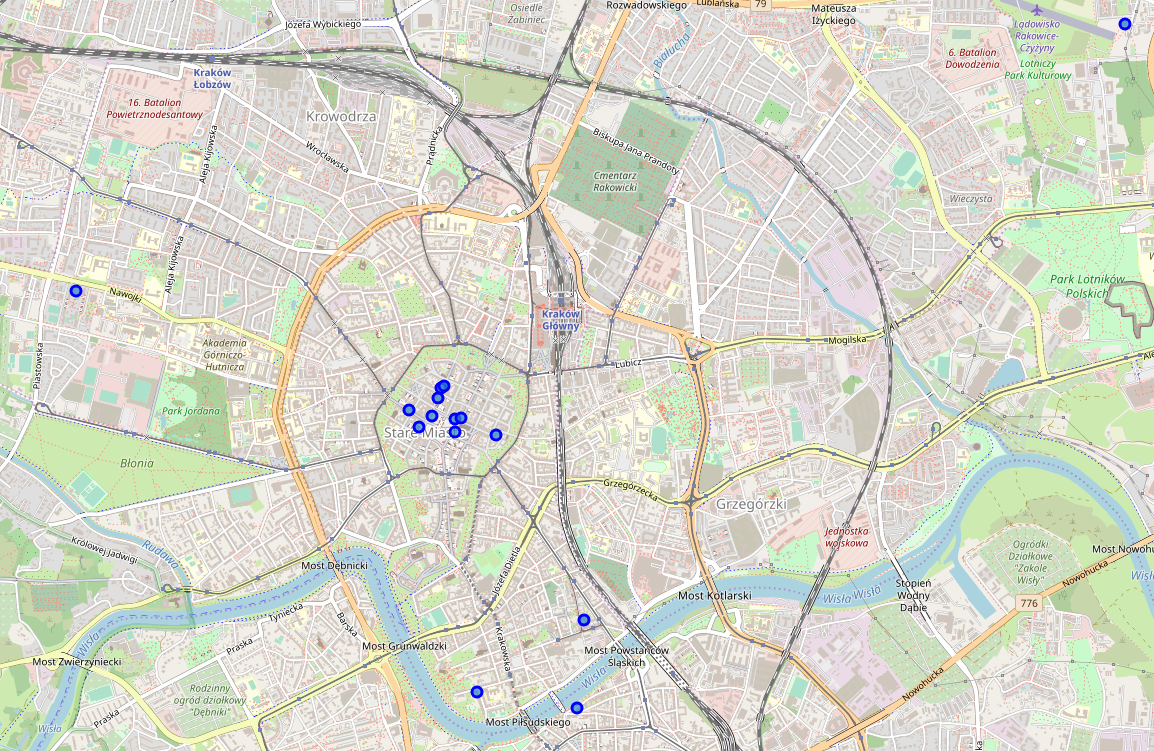
\includegraphics{cracow.png}
\caption{Venues in Cracow}
\end{figure}

    There are 15 music clubs and stores in Cracow. Most of them are
concentrated old town. There are two single outliers - one far east and
one east and a group of three venues Podgorze district.

    Poznan:

    \begin{figure}
\centering
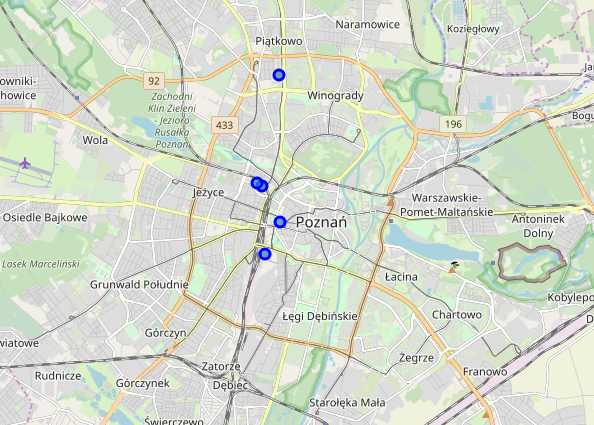
\includegraphics{poznan.png}
\caption{Venues in Poznan}
\end{figure}

    In Poznan there are 5 venues, distributed roughly around straight line.

    Warsaw:

    \begin{figure}
\centering
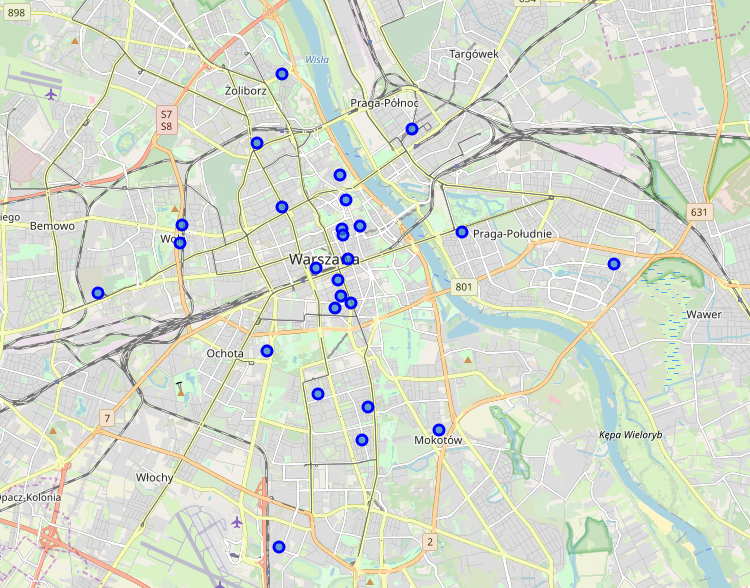
\includegraphics{warsaw.png}
\caption{Venues in Warsaw}
\end{figure}

    There are 26 venues in Warsaw, spread out all over the city in different
districts, with majority of them in the city centre.

    Wroclaw:

    \begin{figure}
\centering
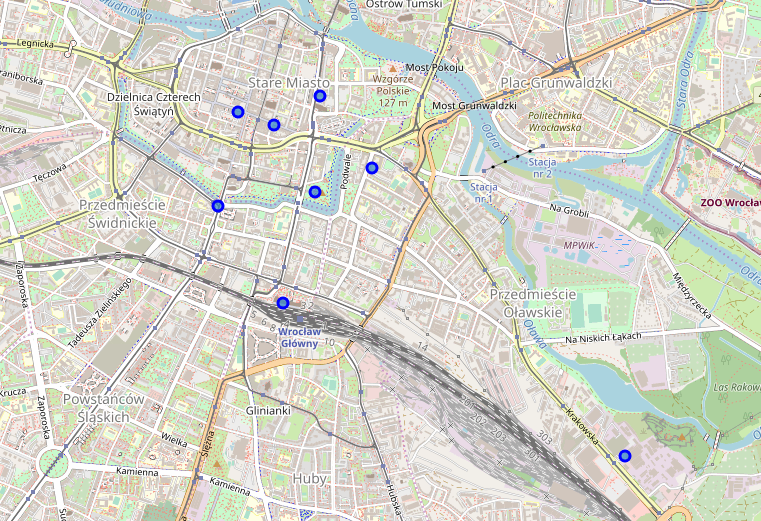
\includegraphics{wroclaw.png}
\caption{Venues in Wroclaw}
\end{figure}

    There are 8 venues of interest in Wroclaw. Their distribution is similar
to Cracow's, most of the venues are located close to Old Town district.

    Clustering

    In order to better compare the cities, the venues were clustered using
k-means clustering by their location. This allows finding the city with
best spatial distribution of venues.

    Cracow:

    \begin{figure}
\centering
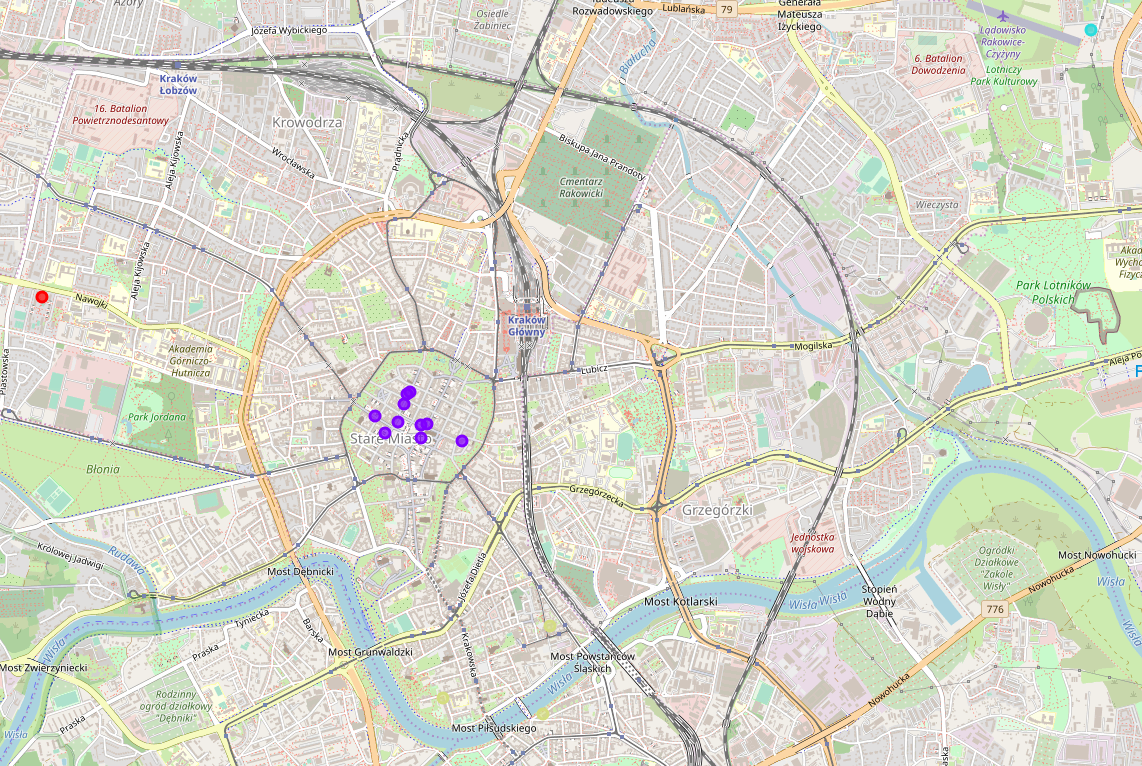
\includegraphics{cracowClusters.png}
\caption{Clusters in cracow}
\end{figure}

    Cracow was divided into 4 clusters, with the most populated containing
10 venues.

    \begin{figure}
\centering
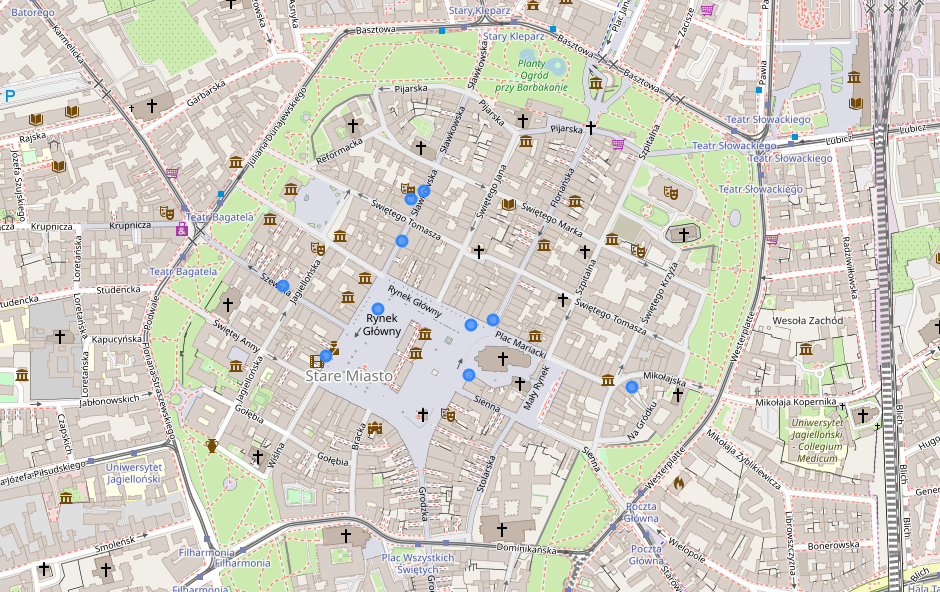
\includegraphics{cracowWin.png}
\caption{Winning cluster in cracow}
\end{figure}

    Poznan:

    \begin{figure}
\centering
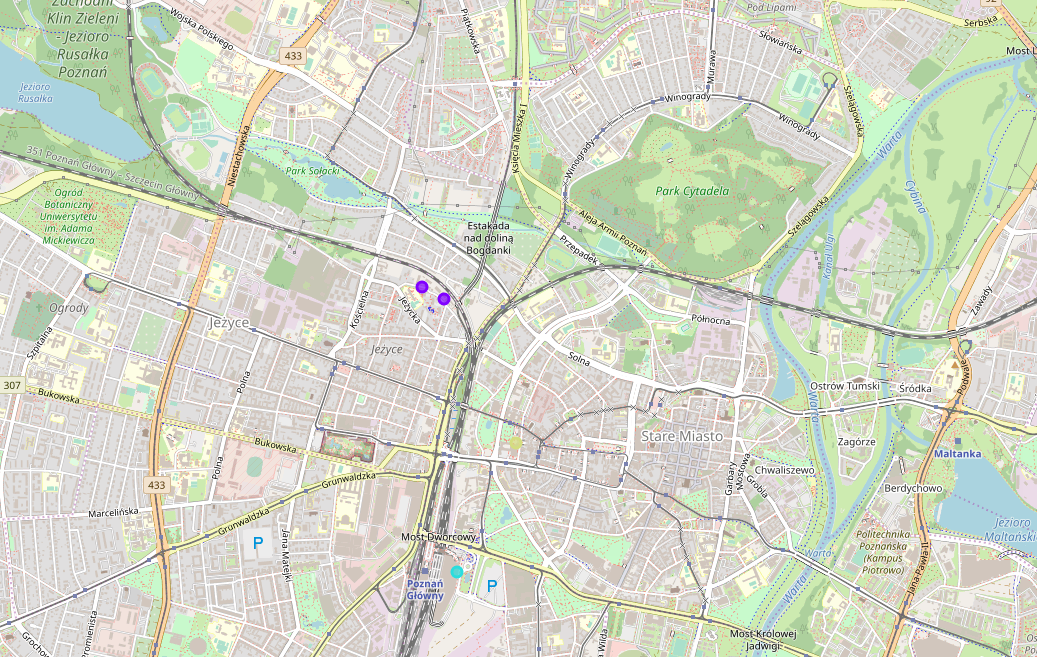
\includegraphics{poznanClusters.png}
\caption{Clusters in Poznan}
\end{figure}

    The winning cluster in Poznan has only 2 venues. At this point it's
obvious that Poznan is the worst city for the objective of this project.

    \begin{figure}
\centering
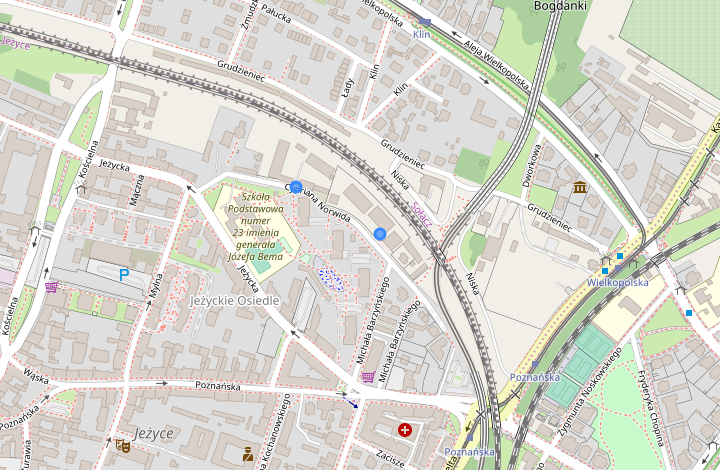
\includegraphics{poznanWin.png}
\caption{Winning cluster in Poznan}
\end{figure}

    Warsaw:

    \begin{figure}
\centering
\includegraphics{warsawClusters.png}
\caption{Winning cluster in Warsaw}
\end{figure}

    The biggest cluster in Warsaw is populated by 15 venues. Warsaw has both
most venues overall and when considering the biggest cluster.

    \begin{figure}
\centering
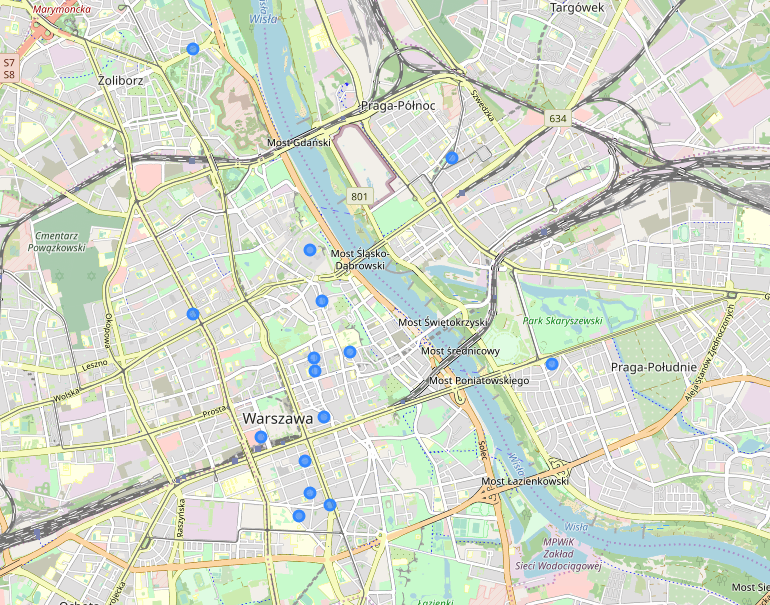
\includegraphics{warsawWin.png}
\caption{Winning cluster in Warsaw}
\end{figure}

    Wroclaw:

    \begin{figure}
\centering
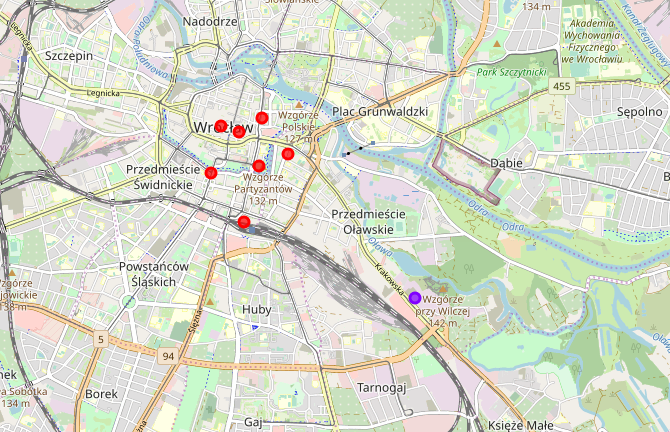
\includegraphics{wroclawClusters.png}
\caption{Clusters in Wroclaw}
\end{figure}

    Biggest cluster in Wroclaw contains 7 venues.

    \begin{figure}
\centering
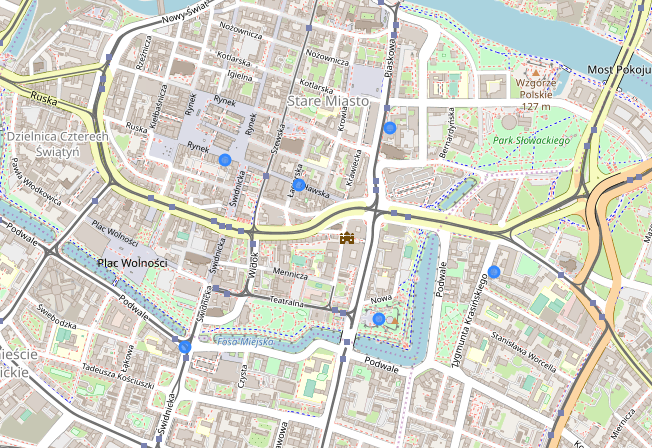
\includegraphics{wroclawWin.png}
\caption{Winning cluster in Wroclaw}
\end{figure}

    Distance within clusters

    The distance within clusters was calculated using city block distance,
as its a more sensible metric than Euclid distance.

    \begin{longtable}[]{@{}lll@{}}
\toprule
City & Number of venues in biggest cluster & Mean
distance\tabularnewline
\midrule
\endhead
Cracow & 10 & 0.024\tabularnewline
Poznan & 2 & 0.021\tabularnewline
Warsaw & 15 & 0.059\tabularnewline
Wroclaw & 7 & 0.018\tabularnewline
\bottomrule
\end{longtable}

    Venue rating in winning clusters

    \begin{longtable}[]{@{}lllll@{}}
\toprule
& Cracow & Poznan & Warsaw & Wroclaw\tabularnewline
\midrule
\endhead
count & 10 & 1 & 5 & 5\tabularnewline
mean & 6.89 & 6.8 & 7.32 & 6.88\tabularnewline
std & 0.86 & NaN & 0.90 & 0.81\tabularnewline
min & 5.8 & 6.8 & 5.8 & 6.1\tabularnewline
25\% & 6.3 & 6.8 & 7.2 & 6.4\tabularnewline
50\% & 6.65 & 6.8 & 7.7 & 6.7\tabularnewline
75\% & 7.775 & 6.8 & 7.9 & 7.0\tabularnewline
max & 8.1 & 6.8 & 8.0 & 8.2\tabularnewline
\bottomrule
\end{longtable}

    A limited number of venues were rated - for example in Warsaw only 5 of
venues were rated compared to 15 venues in cluster. In Cracow all venues
are rated, meaning there are more City Guide users there than other
cities, possibly meaning wider audience.

    \begin{figure}
\centering
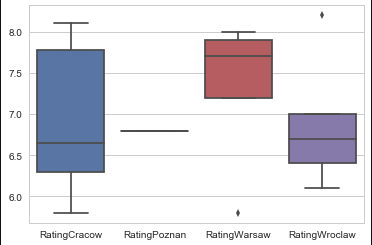
\includegraphics{boxplot.png}
\caption{Boxplot}
\end{figure}

    Cracow and Wroclaw are similar in both spatial distribution of venues
and their ratings. Cracow has twice as much rated venues as Warsaw and
Wroclaw. The median rating is highest in Warsaw, but it may be skewed by
low number of rated venues -- results could change when considering rest
of the venues in cluster.

    \begin{figure}
\centering
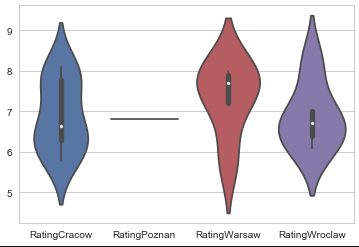
\includegraphics{viol.png}
\caption{Violinplot}
\end{figure}

    Vilion plot shows flatter distributions of venues in Cracaw than in
Warsaw or Wroclaw. The distribution in Warsaw is top heavy, while in
Wroclaw its bottom heavy.

    Discussion

    Poznan lacks music facilities. Cracow and Wroclaw are similar when
considering venues' location and ratings.

While the biggest cluster in Warsaw had 15 venues, only 5 of them were
rated, which may indicate that Cracow is more popular among City Guide
users. Further characterization of an average City Guide user is needed
for more complex conclusions.

Based on this analysis, Cracow is the best city for up-and-coming music
band. There are many music venues -- both clubs and stores with good
ratings. Secondary choice is Warsaw -- it's the biggest city in Poland
with most venues, but due to limited information rating data is
uncertain. While free Foursquare API access gives access to vast amounts
of data, query limit can be an issue.

    Conclusions

    The best city for up-and-coming indie music band is Cracow - it has good
ammount of quality music clubs and stores and is a popular tourist
destination. Close second is Warsaw, thanks to being the biggest city in
Poland it has the most venues overall, but not many of them popular
among City Guide users.

Wroclaw is a smaller city with less venues, but when considering city
centre the results were similar to Cracow.

Poznan is the worst choice - it simply lacks venues.


    % Add a bibliography block to the postdoc
    
    
    
    \end{document}
